\documentclass[11pt]{article}
\usepackage{UF_FRED_paper_style}
\usepackage{wrapfig}

\onehalfspacing

\setlength{\droptitle}{-5em} %% Don't touch

\title{Trabajo 1 - Econometria II
}

\author{Augusto Rico\\% Name author
    \href{mailto:arico@unal.edu.co}{\texttt{arico@unal.edu.co}} %% Email author 1 
\and Mauricio Gomez\\% Name author
    \href{mailto:ivmgomezsi@unal.edu.co}{\texttt{ivmgomezsi@unal.edu.co}} %% Email author 2
\and Diego Barreto\\% Name author
    \href{mailto:dibarretom@unal.edu.co}{\texttt{dibarretom@unal.edu.co}}%% Email author 3
    }

\date{\today}

\begin{document}

\setstretch{.8} %% Don't touch
\maketitle

% %%%%%%%%%%%%%%%%%%%%%%%%%%%%%%%%%%%%%%%%%%%%%%%%%%%%%%%%%%
% %%%%%%%%%%%%%%%%%%%%%%%%%%%%%%%%%%%%%%%%%%%%%%%%%%%%%%%%%%
% BODY OF THE DOCUMENT
% %%%%%%%%%%%%%%%%%%%%%%%%%%%%%%%%%%%%%%%%%%%%%%%%%%%%%%%%%%
% %%%%%%%%%%%%%%%%%%%%%%%%%%%%%%%%%%%%%%%%%%%%%%%%%%%%%%%%%%

% --------------------
\section{Introduccion}
% --------------------

    El objetivo principal de este estudio es demostrar la aplicabilidad de la metodología de Box-Jenkins en la construcción de modelos ARMA (p,q) y ARIMA (p,d,q) en series de tiempo. Para este fin, se utilizará una serie histórica de exportaciones mensuales de petróleo del DANE desde 1982 hasta la fecha actual, compuesta por 372 observaciones. En este trabajo se presentará un análisis detallado del comportamiento de la serie en las cuatro etapas del modelo, que incluyen la identificación, la estimación, la verificación y el pronóstico. A través de este enfoque, se buscará obtener un modelo preciso y confiable que pueda proporcionar información valiosa para la toma de decisiones en el ámbito económico.\\
    En el siguiente gráfico se muestra el comportamiento de la serie durante el periodo de tiempo seleccionado:


\begin{center}
    \begin{figure}[!ht]
      \centering
      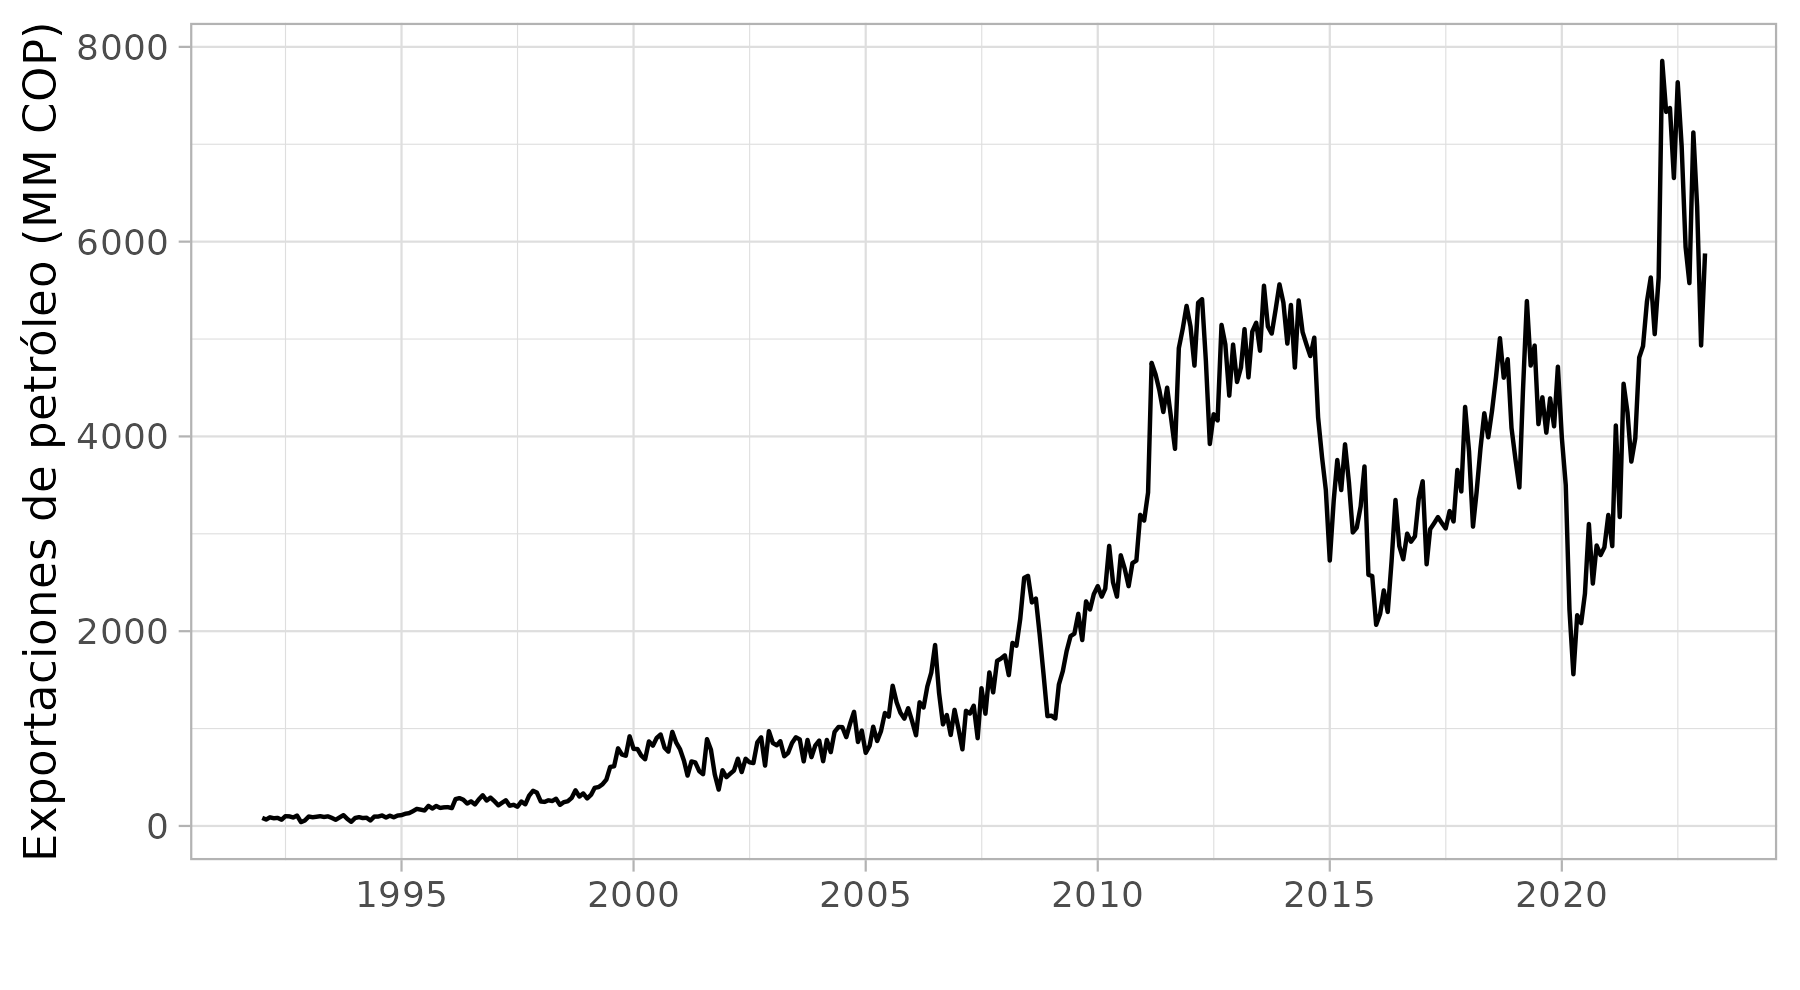
\includegraphics[width=12cm, height=5cm]{Imagenes/ts.png}
      \caption{serie histórica mensual de exportaciones de petróleo de Colombia en miles de millones de pesos colombianos (MM COP) desde 1992 hasta 2023}
      \vspace{0cm}
    \end{figure}
  \end{center}
  
\section{Identificacion de modelo ARMA}

    Para identificar y modelar una serie de tiempo univariada mediante la metodología Box-Jenkins, es necesario que la serie sea estacionaria en covarianza y, por lo tanto, que satisfaga las propiedades de este tipo de series. Para lograr esto, es necesario realizar algunos procedimientos previos:
    \begin{itemize}
        \item Verificar que la serie sea estacionaria en varianza, es decir, que tenga una varianza constante. Si la serie no es constante, se puede aplicar una transformación, como la función logarítmica, para estabilizar la varianza de la serie de tiempo.
        \item Si la serie tiene una tendencia estocástica, se debe aplicar el operador de diferencia para diferenciar la serie y hacerla estacionaria.   
    \end{itemize}
    Para determinar si la serie presenta estacionariedad débil, se pueden analizar la función de autocorrelación simple (FAC) y la función de autocorrelación parcial (FACP).\\~\\
    
\begin{wrapfigure}{l}{8cm}
  \centering
  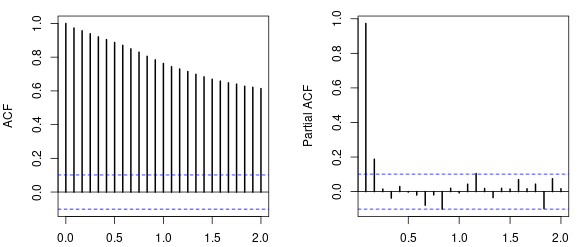
\includegraphics[width=8cm, height=3cm]{Imagenes/acf_pacf1.png}
\end{wrapfigure}
    
    Podemos observar que la función de autocorrelación (FAC) presenta un decaimiento lento hacia cero, lo que sugiere que la serie no es estacionaria en sentido débil. Para comprobar esta hipótesis, se realizó la prueba de Dickey-Fuller, la cual mostró la presencia de una raíz unitaria y, por lo tanto, de no estacionariedad en la serie.\\~\\
    Para poder continuar con la aplicación de la metodología Box-Jenkins, es necesario eliminar las raíces unitarias de la serie. Esto se puede lograr mediante la diferenciación, que también ayuda a estabilizar la varianza de la serie. En este caso, se aplicó la diferenciación de logaritmos a la serie, obteniendo así la serie transformada que muestra la siguiente gráfica y que debe ser interpretada como una tasa de crecimiento:
    
    \begin{center}
        \begin{figure}[!ht]
        \centering
        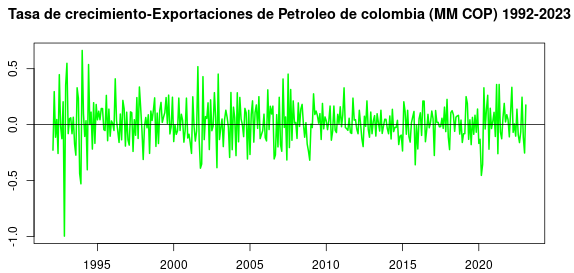
\includegraphics[width=12cm, height=5cm]{Imagenes/creci_ts.png}
        \end{figure}
    \end{center}

    Con el modelo diferenciado, podemos obtener las siguientes funciones ACF y PACF, en 
\begin{wrapfigure}{l}{8cm}
  \centering
  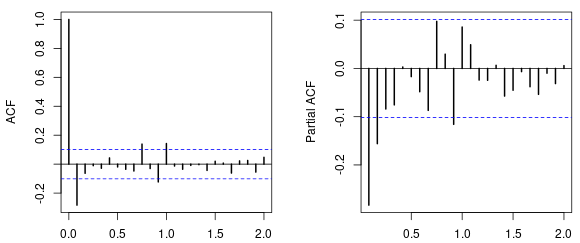
\includegraphics[width=8cm, height=3cm]{Imagenes/acf_pacf2.png}
\end{wrapfigure}

la cual observa una rápida disminución del ACF a cero, lo que indica que la serie es estacionaria en sentido débil. Además, se realizó una prueba de raíces unitarias que confirmó lo observado en la gráfica.\\

En consecuencia, podemos proceder a buscar los grados del modelo ARIMA (p,d,q). Dado que se requirió una diferenciación para satisfacer las condiciones, el grado (d) es igual a 1. Para identificar los grados de AR(p) y MA(q), utilizaremos los valores mínimos obtenidos por el AIC y el BIC y limitaremos nuestra búsqueda a un máximo de 6 rezagos para cada uno. Los valores mínimos obtenidos son los siguientes:

\begin{minipage}{0.5\textwidth}
\begin{flushleft}
~\\adicionalmente se buscó la recomendación del modelo SARIMA utilizando los criterios stepwise y search. El método recomendó utilizar un modelo ARIMA(0,1,1) con estacionalidad (2,0,0). optando asi por el modelo ARIMA(0,1,1) que también fue
\end{flushleft}
\end{minipage}
\hfill
\begin{minipage}{0.5\textwidth}
    \centering
    \begin{tabular}{rrrrrr}
    \hline  Criterio & p & d & q & AIC & BIC \\ 
    \hline
    AIC & 4 & 1 & 2 & -242.31 & -214.86 \\ 
    BIC & 0 & 1 & 1 & -233.32 & -225.48 \\ 
    AIC & 4 & 0 & 3 & -243.33 & -208.04 \\ 
    BIC & 0 & 0 & 1 & -235.35 & -223.59 \\ 
    \hline
    \end{tabular}
\end{minipage}

seleccionado por el criterio BIC, priorizando los modelos con series diferenciadas y parsimoniosos. teniendo en cuenta que uno de nuestros objetivos en este trabajo es pronosticar, y por lo tanto, necesitamos un modelo capaz de generalizar bien con nuevos datos, en lugar de ajustarse únicamente a los datos de entrenamiento. Por lo tanto, evitamos utilizar un modelo demasiado complejo que solo se ajustaría bien a los datos utilizados para crear el modelo.

\section{Estimación de parámetros}
Después de identificar la serie, se procede a estimar su modelo ARIMA utilizando los criterios de información AIC y BIC, priorizando este último como se explicó anteriormente. Sin embargo, si los supuestos de ruido blanco en los residuales del modelo no se cumplen, se deben considerar los modelos seleccionados por AIC o, en su defecto, modelos ARIMA con órdenes más altos de los polinomios autorregresivos y promedios móviles (p y q).

Una vez identificado y seleccionado el modelo ARIMA, se debe proceder a la estimación del mismo utilizando los datos de la serie de tiempo. El método más comúnmente utilizado para estimar los parámetros de una serie de tiempo mediante la metodología Box-Jenkins es la estimación por máxima verosimilitud. Para llevar a cabo esta estimación, se utilizó la función arima del paquete forecast, la cual es capaz de modelar el componente estacional de la serie.\footnote{por el tamaño la tabla se encuentra en anexos}

Aunque la significancia de las variables no es algo relevante en este tipo de modelos, la mayoría de los componentes de los modelos ARMA y ARIMA obtenidos por los criterios AIC y BIC son significativos. Esto nos indica que la selección de parámetros fue adecuada, ya que las estimaciones manuales también contienen valores significativos en sus componentes AR y MA.

\section{Verificación de supuestos\protect\footnotemark}
\footnotetext{En lo siguiente se presentará la validación únicamente de los supuestos del modelo seleccionado ARIMA(0,1,1)(2,0,0); no obstante, se realizaron pruebas en todos los modelos.}
  
Después de haber estimado los modelos seleccionados, es crucial validar los supuestos utilizados para obtener un pronóstico preciso de la serie de tiempo. Los supuestos principales que se deben cumplir son la no autocorrelación de los errores, la homocedasticidad y la normalidad. Por lo general, se utilizó como máximo una cuarta parte de las observaciones como número de rezagos.

En un modelo ARIMA, el supuesto más importante a validar es que los residuos estimados se comporten como un ruido blanco, lo que significa que deben tener una media de cero, una varianza constante y una covarianza de cero. Por lo tanto, es necesario realizar pruebas formales para validar estos supuestos y asegurarse de que los resultados obtenidos sean precisos y confiables.


    
\subsection{Prueba de correlación serial en los residuales}
    Se realizan las pruebas Box-Pierce y Ljung-Box, sobre un 1/4 de la muestra, pero también para rezagos de 20 y 30 periodos, obteniendo que se acepta la hipotesis nula, dado que el P-value $>$ 0.05, por tanto el modelo no presenta autocorrelacion.

\begin{table}[!ht]
    \begin{center}
        \begin{tabular}{l|lll|lll|}
            \cline{2-7}
                & \multicolumn{3}{c|}{Box-Pierce} & \multicolumn{3}{c|}{Ljung-Box} \\ 
            \cline{2-7} 
                & \multicolumn{1}{l|}{Lag(20)} & \multicolumn{1}{l|}{Lag(30)} & Lag(93) & \multicolumn{1}{l|}{Lag(20)} & \multicolumn{1}{l|}{Lag(30)} & Lag(93) \\ 
            \cline{2-7} 
            P-value & \multicolumn{1}{l|}{0.567329} & \multicolumn{1}{l|}{0.672466} & 0.98623 & \multicolumn{1}{l|}{0.530397} & \multicolumn{1}{l|}{0.608956} & 0.917633 \\ 
            \cline{2-7} 
        \end{tabular}
    \end{center}
\end{table}
    

\subsection{Prueba de Heterocedasticidad en los residuales}
\begin{flushleft}
    Este tipo de prueba se basa en la premisa de que si los residuos son heterocedásticos, entonces los residuos al cuadrado deben presentar correlación. Los métodos más comunes para realizar esta prueba son el Test Pormenteau y el Test tipo multiplicadores de Lagrange. Si se rechaza la hipótesis nula (H0) en cualquiera de los dos casos, se concluye que los residuos son heterocedásticos.
\end{flushleft}
    \begin{center}
        \begin{figure}[!ht]
        \centering
        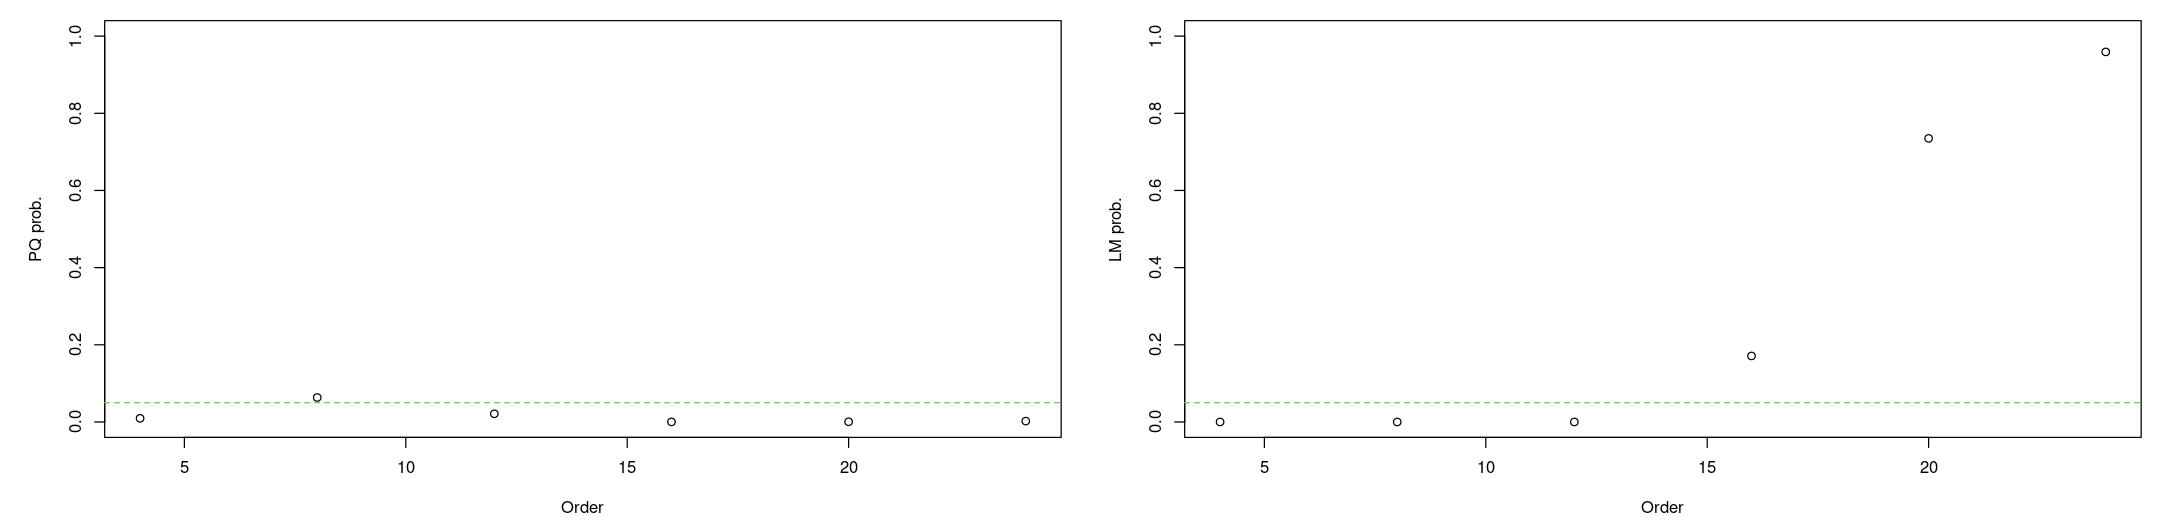
\includegraphics[width=16cm, height=4cm]{Imagenes/Heterocedasticidad.png}
        % \caption{test de efectos ARCH de los residuales}
        \vspace{0cm}
        \end{figure}
    \end{center}
\begin{flushleft}
    En la gráfica se puede observar la presencia de heterocedasticidad en los residuos. Sin embargo, es importante tener en cuenta que las pruebas estadísticas para detectar heterocedasticidad no siempre proporcionan una clara indicación sobre la magnitud del problema en la serie. Por esta razón, es recomendable realizar un análisis adicional para determinar la presencia y la severidad de la heterocedasticidad en la serie. Una opción común es calcular la función de autocorrelación (FAC) y la función de autocorrelación parcial (FACP) de los residuos al cuadrado del modelo ARIMA.
\end{flushleft}

\begin{wrapfigure}{l}{8cm}
    \centering
    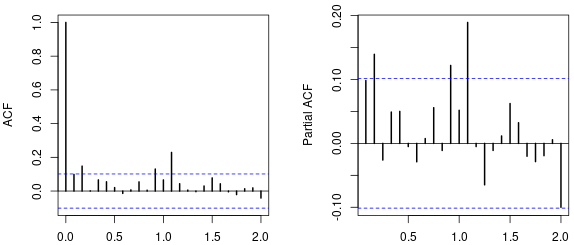
\includegraphics[width=8cm, height=3cm]{Imagenes/acf_pacf_res.png}
  \end{wrapfigure}  
Aunque se observan algunos valores atípicos, éstos no parecen ser generalizados y es posible que estén relacionados con la estacionalidad de los datos. Por lo tanto, es recomendable continuar con el modelo aunque no cumpla plenamente con este supuesto. Sin embargo, se debe tener precaución y verificar si estos valores atípicos afectan significativamente los resultados del modelo.

\subsection{Prueba de normalidad en los residuales}
    Se llevó a cabo la prueba de Jarque-Bera para verificar el supuesto de normalidad. Sin embargo, debido a que el valor p es prácticamente cero, se debe rechazar este supuesto.

\begin{wrapfigure}{l}{4cm}
  \centering
  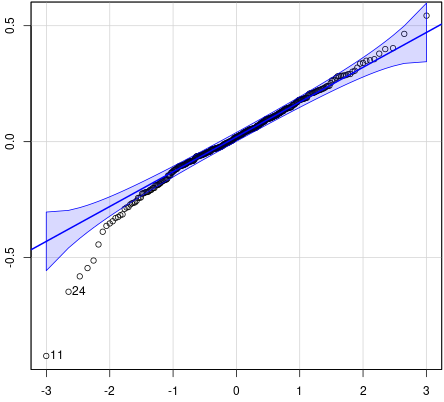
\includegraphics[width=4cm, height=4cm]{Imagenes/normalidad.png}
\end{wrapfigure}
 Cabe señalar que, al igual que con el supuesto de heterocedasticidad, esta prueba no indica la magnitud del problema ni si se presenta en zonas específicas. 

En este sentido, es útil complementar el análisis con una gráfica que permita visualizar la distribución de los datos y tener una intuición sobre la posible presencia de valores atípicos o desviaciones significativas de la normalidad.

Como se puede observar en la gráfica, los problemas de normalidad parecen concentrarse al inicio de la serie. Si bien esto podría afectar en cierta medida el modelo, es importante tener en cuenta que este comportamiento podría deberse al incremento abrupto en el precio del petróleo registrado en la época inicial de los datos. En efecto, mientras que el precio rondaba los 15 dólares en aquel momento, durante el año 2008 llegó a alcanzar incluso los 150 dólares.

\subsection{Corrección de violación de supuestos}
La corrección del supuesto de normalidad en la modelación de series de tiempo se puede lograr mediante la aplicación de transformaciones de los datos, la utilización de modelos de distribución alternativos que se ajusten mejor a los datos o métodos de simulación como el bootstrapping. En cuanto a la corrección del supuesto de homocedasticidad, se pueden emplear transformaciones de los datos, modelos ARCH que permiten modelar la varianza de los residuos, o modelos GARCH que permiten modelar tanto la media como la varianza de los residuos. Es importante considerar que la selección del método adecuado dependerá de las características y patrones específicos de los datos de la serie de tiempo.

\subsection{conclusiones validacion}
A partir de los resultados obtenidos, se puede concluir que no es posible verificar el cumplimiento de los supuestos de normalidad y homocedasticidad en los errores del modelo seleccionado, ya que se rechazan las hipótesis nulas a partir de los p-valores reportados. No obstante, es importante destacar que el modelo cumple con el supuesto de no correlación de los errores, lo que sugiere que estos pueden ser utilizados en la fase de pronóstico de la serie. En todo caso, es recomendable tener precaución y considerar la posibilidad de explorar otros modelos o aplicar técnicas de transformación de datos si se identifica alguna fuente de sesgo o heterogeneidad en los errores.

\section{Uso del modelo (Pronostico)}
    Esta última fase tiene como propósito aplicar el modelo seleccionado en la investigación de la serie de tiempo. En este caso, se va a hacer un pronóstico de las exportaciones de petróleo en Colombia para los próximos 10 períodos, es decir, desde marzo de 2023 hasta diciembre de 2023, utilizando el modelo ARIMA (0,1,1)\footnote{tabla en el anexo}, estimacion que puede observarse en la siguiente grafica
    \begin{center}
        \begin{figure}[!ht]
        \centering
        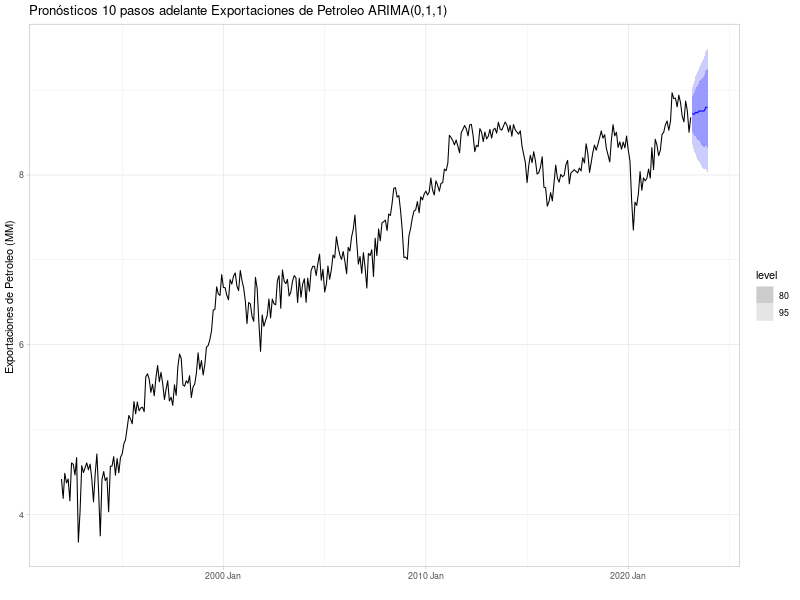
\includegraphics[width=16cm, height=8cm]{Imagenes/Pred.png}
        % \caption{Pronostico 10 periodos adelante}
        \end{figure}
    \end{center}
    finalmente, se observa, el ajuste dentro de la muestra del modelo diferenciado manualmente:
    \begin{center}
        \begin{figure}[!ht]
        \centering
        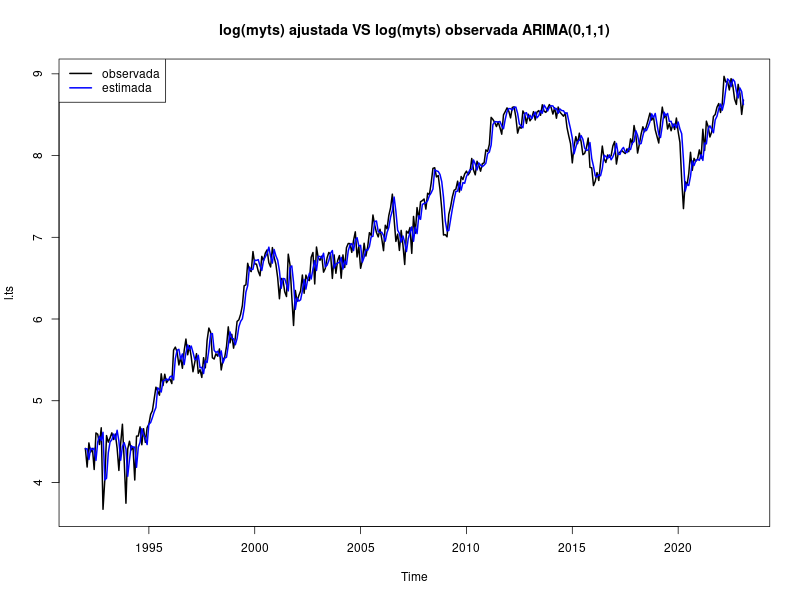
\includegraphics[width=16cm, height=8cm]{Imagenes/ajuste.png}
        \caption{Serie de Tiempo Ajustada vs Observada}
        \end{figure}
    \end{center}

del cual se puede afirmar que el modelo diferenciado manualmente presenta un ajuste adecuado dentro de la muestra. La inspección visual de los gráficos de residuos y el análisis de la prueba Ljung-Box respaldan esta afirmación. Sin embargo, es importante señalar que el ajuste en muestra no necesariamente garantiza un buen desempeño en la predicción fuera de la muestra. Por lo tanto, se deben realizar pruebas adicionales para evaluar la capacidad predictiva del modelo y verificar si cumple con los objetivos de la investigación.

\section{Conclusiones finales}
 la metodologia Box-Jenkings es una herramienta sumamente valiosa para la construccion de series de tiempo estacionarias.
 Esta tecnica proporciona un analisis detallado de los datos que permite realizar pronosticos precisos y buscar las formas de de minimizar el termino de error en los modelos propuestos. En relacion a la serie de tiempo que se utilizo en este estudio, se puede observar que el crecimiento de las expotaciones de petroleo en Colombia sigue una tendencia ascendente, lo cual coincide con el crecimiento del sector economico en los ultimos años del pais. Sin embargo, se hace necesario abordar en futuras investigaciones la heterocedasticidad y normalidad de los datos para lograr una mejor calibracion del modelo, por leves datos atipicos que presento la serie de tiempo.

\newpage

\nocite{*}
\bibliography{references.bib}

\newpage
\section{anexos}

\begin{table}[!htbp] \centering 
  \caption{Estimacion de parametros} 
  \label{} 
\begin{tabular}{@{\extracolsep{5pt}}lcccc} 
\\[-1.8ex]\hline 
\hline \\[-1.8ex] 
\\[-1.8ex] & \multicolumn{2}{c}{l.ts} & \multicolumn{2}{c}{dl.ts} \\ 
 & ARIMA (4,1,2) & ARIMA (0,1,1) & ARMA (4,3) & AR(1) \\ 
\\[-1.8ex] & (1) & (2) & (3) & (4)\\ 
\hline \\[-1.8ex] 
 ar1 & $-$0.699$^{***}$ &  & $-$0.446$^{*}$ &  \\ 
  & (0.059) &  & (0.261) &  \\ 
  & & & & \\ 
 ar2 & $-$1.196$^{***}$ &  & $-$1.026$^{***}$ &  \\ 
  & (0.061) &  & (0.197) &  \\ 
  & & & & \\ 
 ar3 & $-$0.412$^{***}$ &  & $-$0.145 &  \\ 
  & (0.060) &  & (0.282) &  \\ 
  & & & & \\ 
 ar4 & $-$0.215$^{***}$ &  & $-$0.150 &  \\ 
  & (0.053) &  & (0.102) &  \\ 
  & & & & \\ 
 ma1 & 0.383$^{***}$ & $-$0.352$^{***}$ & 0.109 & $-$0.379$^{***}$ \\ 
  & (0.035) & (0.053) & (0.266) & (0.053) \\ 
  & & & & \\ 
 ma2 & 0.959$^{***}$ &  & 0.842$^{***}$ &  \\ 
  & (0.022) &  & (0.115) &  \\ 
  & & & & \\ 
 sar1 &  & 0.141$^{**}$ &  &  \\ 
  &  & (0.055) &  &  \\ 
  & & & & \\ 
 sar2 &  & 0.048 &  &  \\ 
  &  & (0.058) &  &  \\ 
  & & & & \\ 
 ma3 &  &  & $-$0.278 &  \\ 
  &  &  & (0.266) &  \\ 
  & & & & \\ 
 intercept &  &  & 0.012$^{**}$ & 0.012$^{**}$ \\ 
  &  &  & (0.005) & (0.006) \\ 
  & & & & \\ 
Observations & 373 & 373 & 373 & 373 \\ 
\hline \\[-1.8ex] 
\textit{Notes:} & \multicolumn{4}{l}{$^{***}$Significant at the 1 percent level.} \\ 
 & \multicolumn{4}{l}{$^{**}$Significant at the 5 percent level.} \\ 
 & \multicolumn{4}{l}{$^{*}$Significant at the 10 percent level.} \\ 
\end{tabular} 
\end{table}

\begin{center}
    \begin{figure}[htbp]
        \centering
        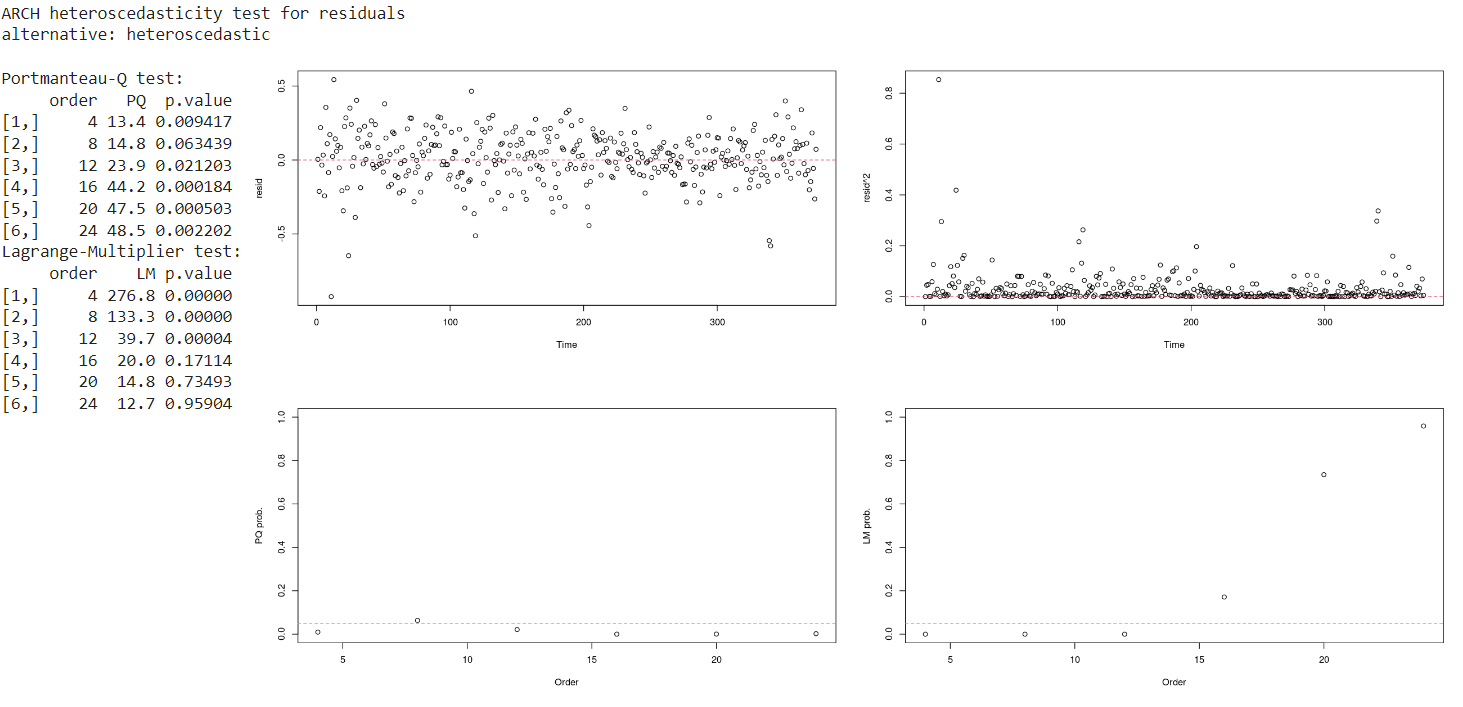
\includegraphics[scale=0.5]{Imagenes/Hetero.png}
        \caption{test de efectos ARCH de los residuales}
    \end{figure}
\end{center}
    
\begin{center}
    \begin{figure}[htbp]
        \centering
        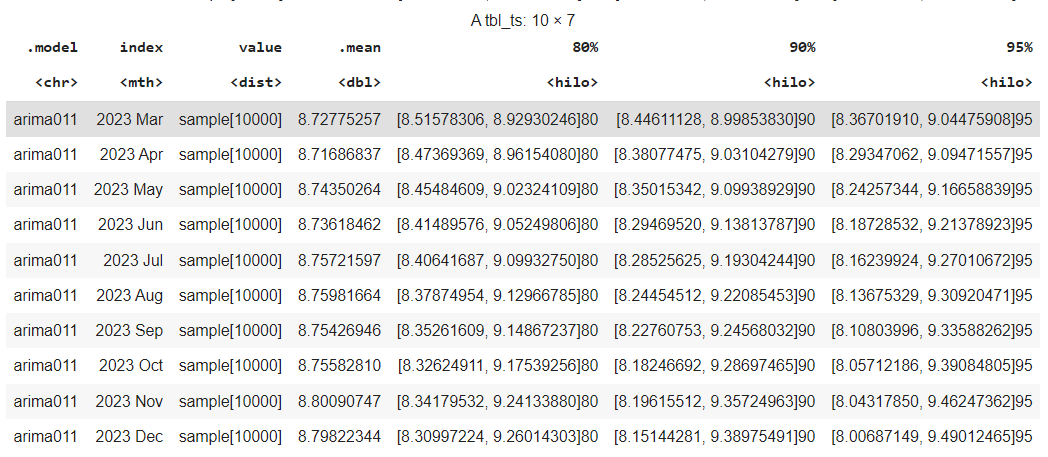
\includegraphics[scale=0.5]{Imagenes/Pro-interv.png}
        \caption{Pronosticos puntuales e intervalos de prediccion, 10 periodos adelante}
    \end{figure}
\end{center}

\end{document}